\documentclass[12pt,aspectratio=169]{beamer}
\usepackage[T1]{fontenc}
\usepackage{lmodern,amsmath,amssymb,booktabs,tikz,graphicx}
\usetikzlibrary{arrows.meta,positioning,calc}
\definecolor{Ink}{HTML}{17324D}
\definecolor{Teal}{HTML}{007F7A}
\definecolor{Muted}{HTML}{556574}
\definecolor{Paper}{HTML}{FAFAF7}
\definecolor{Rust}{HTML}{AD532E}
\definecolor{Gold}{HTML}{B38630}
\setbeamercolor{background canvas}{bg=Paper}
\setbeamercolor{normal text}{fg=Ink}
\setbeamercolor{frametitle}{fg=Ink}
\setbeamercolor{structure}{fg=Teal}
\setbeamercolor{alerted text}{fg=Rust}
\setbeamerfont{frametitle}{size=\LARGE,series=\bfseries}
\setbeamertemplate{navigation symbols}{}
\setbeamersize{text margin left=9mm,text margin right=9mm}
\setbeamertemplate{frametitle}{\par\vspace{2mm}\insertframetitle\par\vspace{1mm}{\color{Gold}\rule{14mm}{1pt}}}
\setbeamertemplate{footline}{\hspace{9mm}\scriptsize\color{Muted}\insertsectionhead\hfill\insertframenumber\hspace{9mm}\vspace{4mm}}
\hypersetup{colorlinks=true,urlcolor=Teal,linkcolor=Muted,pdfauthor={}}
\newcommand{\point}[1]{\par\vspace{3mm}{\large #1\par}}
\newcommand{\eqnote}[1]{\par\vspace{2mm}{\small\color{Muted}#1\par}}
\newcommand{\smalltext}[1]{\eqnote{#1}}
\newcommand{\insight}[1]{\par\vspace{2mm}{\color{Teal}\bfseries #1}\par}
\newcommand{\identity}{\text{\scriptsize accounting identity}}
\newcommand{\policy}{R^{\mathrm{policy}}}
\newcommand{\loanrate}{R^{\mathrm{loan}}}
\newcommand{\nominal}{R^{\mathrm{nom}}}
\newcommand{\realrate}{R^{\mathrm{real}}}
\newcommand{\neutral}{R^{\mathrm{neutral}}}
\newcommand{\spot}[1]{R^{\mathrm{spot}}(#1)}
\newcommand{\forward}[2]{R^{\mathrm{forward}}(#1,#2)}
\newcommand{\bondyield}{R^{\mathrm{bond}}}
\newcommand{\bondrate}[1]{R^{\mathrm{bond}}(#1)}
\AtBeginDocument{\setlength{\abovedisplayskip}{5pt}\setlength{\belowdisplayskip}{5pt}\setlength{\abovedisplayshortskip}{3pt}\setlength{\belowdisplayshortskip}{3pt}}

\hypersetup{pdftitle={Economics and Finance for Mathematicians: Currency crises and the euro}}
\begin{document}

% Slide 1: Currency crises and the euro

\begin{frame}[plain]
{\color{Teal}\large ECONOMICS AND FINANCE\quad /\quad 06}\par\vspace{9mm}{\Huge\bfseries Currency crises and the euro}\par\vspace{7mm}{\Large How can balance sheets and expectations turn a funding shock into a crisis?}
\end{frame}

% Slide 2: Today’s route

\begin{frame}{Today’s route}
\point{Currency mismatches can reverse the trade benefits of depreciation.}\point{Pegs can fail through deteriorating fundamentals or coordination.}\point{A currency union changes the adjustment tools and financial risks.}
\end{frame}

% Slide 3: Balance-sheet exposure
\section[Balance-sheet exposure]{Balance-sheet exposure}
\begin{frame}[plain]
{\color{Gold}\large LECTURE 6}\par\vspace{9mm}{\Huge\bfseries Balance-sheet exposure}\par\vspace{7mm}{\Large Why can a weaker currency reduce domestic demand?}
\end{frame}

% Slide 4: A firm borrows dollars but earns home currency

\begin{frame}{A firm borrows dollars but earns home currency}
\begin{center}\begin{tabular}{@{}lll@{}}\toprule \textbf{Balance sheet, home currency} & \textbf{Before} & \textbf{After depreciation}\\\midrule Operating assets & 200 & 200\\[2mm]
USD debt: one dollar & 150 & 180\\[2mm]
Equity & 50 & 20\\\bottomrule\end{tabular}\end{center}\eqnote{Home per USD rises 20\%, from 150 to 180. Asset values are held fixed.}
\end{frame}

% Slide 5: Trade and financial channels can oppose each other

\begin{frame}{Trade and financial channels can oppose each other}
\begin{center}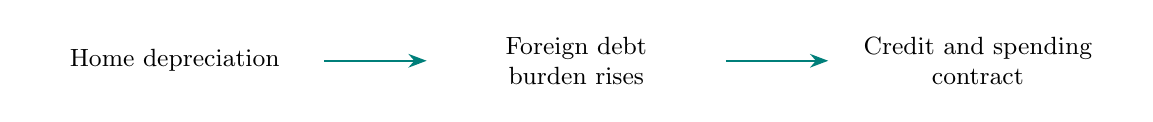
\begin{tikzpicture}[>=Stealth,every node/.style={font=\small,align=center,text width=3.5cm}]\node at (0.0,0){Home depreciation};\node at (5.1,0){Foreign debt\\burden rises};\node at (10.2,0){Credit and spending\\contract};\draw[->,Teal,thick] (1.9,0)--(3.1999999999999997,0);\draw[->,Teal,thick] (7.0,0)--(8.299999999999999,0);\end{tikzpicture}\end{center}\point{A currency move changes liabilities as well as product prices.}
\end{frame}

% Slide 6: Debt and equity share bad states differently

\begin{frame}{Debt and equity share bad states differently}
\begin{center}\begin{tabular}{@{}p{.30\textwidth}p{.62\textwidth}@{}}\toprule \textbf{Foreign finance} & \textbf{What happens in a recession?}\\\midrule Fixed nominal debt & Promised payment initially stays fixed\\[2mm]
Equity ownership & Dividends and market value can absorb losses\\\bottomrule\end{tabular}\end{center}\eqnote{Equity shares risk, while financing terms, control and valuation still matter.}
\end{frame}

% Slide 7: Pegs under pressure
\section[Pegs under pressure]{Pegs under pressure}
\begin{frame}[plain]
{\color{Gold}\large LECTURE 6}\par\vspace{9mm}{\Huge\bfseries Pegs under pressure}\par\vspace{7mm}{\Large When does defending a fixed rate become impossible or too costly?}
\end{frame}

% Slide 8: A first-generation crisis mechanism

\begin{frame}{A first-generation crisis mechanism}
\point{Domestic credit keeps expanding while the peg fixes money demand.}\point{Foreign reserves offset the expansion and decline.}\point{The policy combination eventually cannot continue.}
\end{frame}

% Slide 9: Reserves can be exhausted by an anticipated attack

\begin{frame}{Reserves can be exhausted by an anticipated attack}
\begin{center}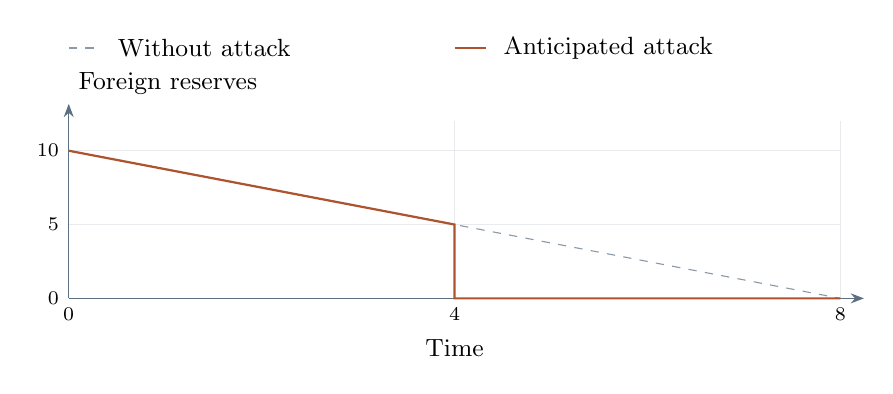
\begin{tikzpicture}[>=Stealth,every node/.style={font=\small}]
\draw[Ink!10] (0.0000,0.0000)--(0.0000,2.2500);\node[below,font=\scriptsize] at (0.0000,0.0000){0};
\draw[Ink!10] (4.9000,0.0000)--(4.9000,2.2500);\node[below,font=\scriptsize] at (4.9000,0.0000){4};
\draw[Ink!10] (9.8000,0.0000)--(9.8000,2.2500);\node[below,font=\scriptsize] at (9.8000,0.0000){8};
\draw[Ink!10] (0.0000,0.0000)--(9.8000,0.0000);\node[left,font=\scriptsize] at (0.0000,0.0000){0};
\draw[Ink!10] (0.0000,0.9375)--(9.8000,0.9375);\node[left,font=\scriptsize] at (0.0000,0.9375){5};
\draw[Ink!10] (0.0000,1.8750)--(9.8000,1.8750);\node[left,font=\scriptsize] at (0.0000,1.8750){10};
\draw[->,Ink!70] (0,0)--(10.100000000000001,0);\draw[->,Ink!70] (0,0)--(0,2.47);
\node[below] at (4.9,-.40){Time};\node[anchor=west] at (0,2.73){Foreign reserves};
\draw[Ink!50,dashed] plot coordinates {(0.0000,1.8750) (9.8000,0.0000)};
\draw[Rust,thick] plot coordinates {(0.0000,1.8750) (4.9000,0.9375) (4.9000,0.0000) (9.8000,0.0000)};
\draw[Ink!50,dashed] (0.0,3.18)--(0.4,3.18);\node[anchor=west,font=\small] at (0.5,3.18){Without attack};
\draw[Rust,thick] (4.9,3.18)--(5.300000000000001,3.18);\node[anchor=west,font=\small] at (5.4,3.18){Anticipated attack};
\end{tikzpicture}\end{center}\eqnote{Schematic path, not a fitted crisis date or empirical reserve series.}
\end{frame}

% Slide 10: A second-generation crisis mechanism

\begin{frame}{A second-generation crisis mechanism}
\point{Defending the peg raises interest rates and domestic economic costs.}\point{Investors’ exit expectations can increase the cost of defence.}\point{The authorities may choose to abandon the peg.}
\end{frame}

% Slide 11: A coordination example

\begin{frame}{A coordination example}
\point{Two large investors can each withdraw 4 units.}\point{The authority can absorb 6 units of withdrawals.}\point{One exit is manageable. Two simultaneous exits break the peg.}
\end{frame}

% Slide 12: The coordination game

\begin{frame}{The coordination game}
\begin{center}\begin{tabular}{@{}lll@{}}\toprule \textbf{Investor 1 / Investor 2} & \textbf{Stay} & \textbf{Exit}\\\midrule Stay & (0, 0) & (0, -1)\\[2mm]
Exit & (-1, 0) & (+2, +2)\\\bottomrule\end{tabular}\end{center}\point{Both staying and both exiting can be equilibria.}
\end{frame}

% Slide 13: A backstop can change incentives

\begin{frame}{A backstop can change incentives}
\point{Credible support can remove the payoff from joining a run.}\point{Support needs resources, legal authority and believable conditions.}\point{A liquidity backstop does not automatically repair insolvency.}
\end{frame}

% Slide 14: Currency unions
\section[Currency unions]{Currency unions}
\begin{frame}[plain]
{\color{Gold}\large LECTURE 6}\par\vspace{9mm}{\Huge\bfseries Currency unions}\par\vspace{7mm}{\Large When is sharing one monetary policy worth the loss of local adjustment?}
\end{frame}

% Slide 15: The benefits and costs of a common currency

\begin{frame}{The benefits and costs of a common currency}
\point{Trade and financial integration reduce conversion costs and currency risk.}\point{A common rate cannot respond separately to every national shock.}\point{Other adjustment channels become more important.}
\end{frame}

% Slide 16: An integration trade-off

\begin{frame}{An integration trade-off}
\begin{center}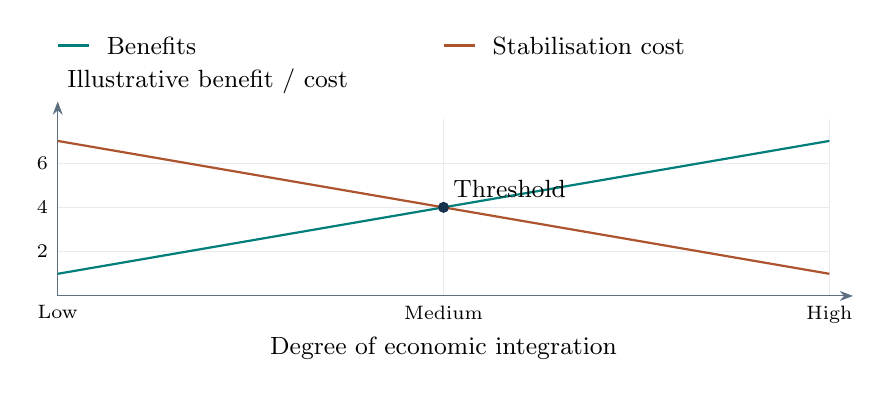
\begin{tikzpicture}[>=Stealth,every node/.style={font=\small}]
\draw[Ink!10] (0.0000,0.0000)--(0.0000,2.2500);\node[below,font=\scriptsize] at (0.0000,0.0000){Low};
\draw[Ink!10] (4.9000,0.0000)--(4.9000,2.2500);\node[below,font=\scriptsize] at (4.9000,0.0000){Medium};
\draw[Ink!10] (9.8000,0.0000)--(9.8000,2.2500);\node[below,font=\scriptsize] at (9.8000,0.0000){High};
\draw[Ink!10] (0.0000,0.5625)--(9.8000,0.5625);\node[left,font=\scriptsize] at (0.0000,0.5625){2};
\draw[Ink!10] (0.0000,1.1250)--(9.8000,1.1250);\node[left,font=\scriptsize] at (0.0000,1.1250){4};
\draw[Ink!10] (0.0000,1.6875)--(9.8000,1.6875);\node[left,font=\scriptsize] at (0.0000,1.6875){6};
\draw[->,Ink!70] (0,0)--(10.100000000000001,0);\draw[->,Ink!70] (0,0)--(0,2.47);
\node[below] at (4.9,-.40){Degree of economic integration};\node[anchor=west] at (0,2.73){Illustrative benefit / cost};
\draw[Teal,thick] plot coordinates {(0.0000,0.2812) (9.8000,1.9688)};
\draw[Rust,thick] plot coordinates {(0.0000,1.9688) (9.8000,0.2812)};
\fill[Ink] (4.9000,1.1250) circle (2pt);\node[above right] at (4.9000,1.1250){Threshold};
\draw[Teal,thick] (0.0,3.18)--(0.4,3.18);\node[anchor=west,font=\small] at (0.5,3.18){Benefits};
\draw[Rust,thick] (4.9,3.18)--(5.300000000000001,3.18);\node[anchor=west,font=\small] at (5.4,3.18){Stabilisation cost};
\end{tikzpicture}\end{center}\eqnote{A schematic OCA trade-off, not a measured threshold for any nation.}
\end{frame}

% Slide 17: A common currency does not make every price identical

\begin{frame}{A common currency does not make every price identical}
\point{Euro-area countries share monetary policy.}\point{Their consumption baskets, energy exposure,\par local taxes and price adjustments still differ.}\eqnote{One currency does not imply one national inflation rate.}
\end{frame}

% Slide 18: Different baskets can produce different inflation

\begin{frame}{Different baskets can produce different inflation}
\begin{center}\begin{tabular}{@{}lll@{}}\toprule \textbf{Hypothetical basket} & \textbf{Country A} & \textbf{Country B}\\\midrule Energy weight & 10\% & 30\%\\[2mm]
Other goods/services weight & 90\% & 70\%\\[2mm]
Energy price increase & 20\% & 20\%\\[2mm]
Other price increase & 2\% & 2\%\\[2mm]
Basket inflation & 3.8\% & 7.4\%\\\bottomrule\end{tabular}\end{center}\eqnote{Same component price increases, different fixed basket weights.}
\end{frame}

% Slide 19: A shared nominal rate can mean different real rates

\begin{frame}{A shared nominal rate can mean different real rates}
\begin{center}\begin{tabular}{@{}lll@{}}\toprule \textbf{Hypothetical comparison} & \textbf{Country A} & \textbf{Country B}\\\midrule Same nominal rate & 4\% & 4\%\\[2mm]
Expected basket inflation & 2\% & 4\%\\[2mm]
Approximate expected real rate & 2\% & 0\%\\\bottomrule\end{tabular}\end{center}\point{The purchasing-power cost depends on expected inflation.}
\end{frame}

% Slide 20: Euro government bonds can also have different yields

\begin{frame}{Euro government bonds can also have different yields}
\point{Same currency, different issuers and credit risk.}\point{Liquidity, collateral value and market conditions also differ.}\eqnote{National inflation is not a mechanical add-on to a euro sovereign yield.\par The plotted ECB AAA curve is a benchmark sample, not every nation\textquotesingle s curve.}
\end{frame}

% Slide 21: Relative prices can adjust without a currency change

\begin{frame}{Relative prices can adjust without a currency change}
\[\Delta\ln q=\pi^{\rm foreign}-\pi^{\rm home}\quad\text{when }E\text{ is fixed}.\]\point{Higher local inflation can create real appreciation inside a currency union.}
\end{frame}

% Slide 22: Banks and sovereigns
\section[Banks and sovereigns]{Banks and sovereigns}
\begin{frame}[plain]
{\color{Gold}\large LECTURE 6}\par\vspace{9mm}{\Huge\bfseries Banks and sovereigns}\par\vspace{7mm}{\Large How can two balance sheets make each other weaker?}
\end{frame}

% Slide 23: Banks transform maturities

\begin{frame}{Banks transform maturities}
\begin{center}\begin{tabular}{@{}ll@{}}\toprule \textbf{Assets} & \textbf{Liabilities}\\\midrule Longer-term loans and securities & Deposits withdrawable on demand\\\bottomrule\end{tabular}\end{center}\point{A solvent bank can lack cash for simultaneous withdrawals.}
\end{frame}

% Slide 24: A sovereign refinancing feedback

\begin{frame}{A sovereign refinancing feedback}
\begin{center}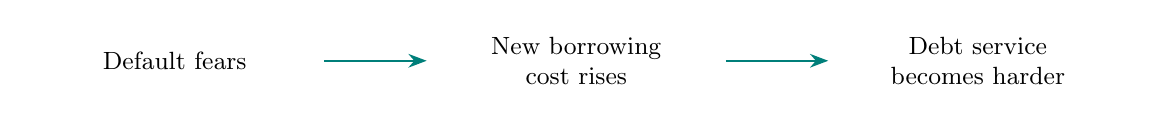
\begin{tikzpicture}[>=Stealth,every node/.style={font=\small,align=center,text width=3.5cm}]\node at (0.0,0){Default fears};\node at (5.1,0){New borrowing\\cost rises};\node at (10.2,0){Debt service\\becomes harder};\draw[->,Teal,thick] (1.9,0)--(3.1999999999999997,0);\draw[->,Teal,thick] (7.0,0)--(8.299999999999999,0);\end{tikzpicture}\end{center}\point{The higher funding cost can make the original fear more plausible.}
\end{frame}

% Slide 25: The bank–sovereign loop

\begin{frame}{The bank–sovereign loop}
\begin{center}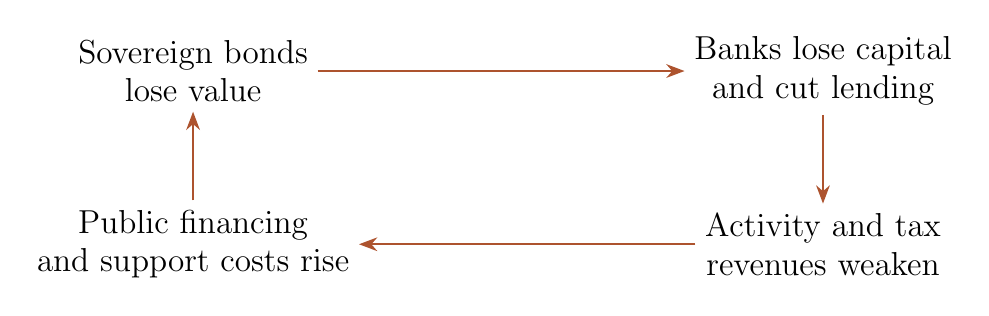
\begin{tikzpicture}[>=Stealth,every node/.style={font=\large,align=center}]\node(A)at(0,1){Sovereign bonds\\lose value};\node(B)at(8,1){Banks lose capital\\and cut lending};\node(C)at(8,-1.2){Activity and tax\\revenues weaken};\node(D)at(0,-1.2){Public financing\\and support costs rise};\draw[->,Rust,thick](A)--(B);\draw[->,Rust,thick](B)--(C);\draw[->,Rust,thick](C)--(D);\draw[->,Rust,thick](D)--(A);\end{tikzpicture}\end{center}
\end{frame}

% Slide 26: A historical backstop: OMT in 2012

\begin{frame}{A historical backstop: OMT in 2012}
\point{The ECB set out its OMT technical framework on 6 September 2012.}\point{Eligible sovereign support required programme conditionality.}\point{The mechanism targeted severe transmission and redenomination fears.}
\end{frame}

% Slide 27: Exercise: liquidity support or a fiscal repair?

\begin{frame}{Exercise: liquidity support or a fiscal repair?}
\point{A bank has sound long-term loans but sudden deposit withdrawals.}\point{A government faces a temporary market closure with credible future surpluses.}\point{Another government cannot plausibly fund its promises in real terms.}
\end{frame}

% Slide 28: Further reading
\section[Reading]{Reading}
\begin{frame}{Further reading}
\point{Dmitriy Sergeyev, Bocconi 30054 course materials.}\point{Krugman, Obstfeld \& Melitz, \emph{International Economics}.}\point{Source links and worked answers accompany each slide in the notes.}
\end{frame}
\end{document}
